\documentclass[a4paper,12pt]{report}
\usepackage[spanish,mexico]{babel}
\usepackage[utf8]{inputenc}
\usepackage[T1]{fontenc}
\usepackage{amsmath}
\usepackage{amssymb}
\usepackage{wasysym}
\usepackage[dvipsnames,pdftex]{color}
\usepackage[x11names]{xcolor}
\usepackage{tikz, tkz-euclide}
\usepackage[american]{circuitikz}
\usepackage{siunitx}
\usetikzlibrary{arrows}
\usepackage[colorinlistoftodos]{todonotes}
%\usepackage[left=2cm,right=1.5cm,top=1cm,bottom=1cm]{geometry}
%\usepackage{helvet}
%\renewcommand{\familydefault}{\sfdefault}
\setlength{\oddsidemargin}{0in}
\usepackage{geometry}
\geometry{a4paper, total = {180mm,270mm},
			left = 25mm, top = 20mm,
            right=15mm,bottom=20mm,%
            footskip=10mm}
\usepackage{float} 
% \setlength{\topmargin}{0in}
% \setlength{\voffset}{-0.5in}
% \setlength{\hoffset}{0.3in}
% \setlength{\textheight}{700pt}
% \setlength{\textwidth}{440pt}
% \setlength{\topskip}{0in}
% \setlength{\parskip}{2ex}
 \renewcommand{\baselinestretch}{1.5}
\usepackage{diagbox}
\usepackage{array}
\usepackage{listings}
\usepackage{caption}
%%% comandos definidos por el usuario
\begin{document}
\setcounter{page}{1}
\pagenumbering{roman}
\thispagestyle{empty}
\begin{center}
{\huge UNIVERSIDAD NACIONAL DE INGENIERÍA}\\[0.9cm]
{\Large FACULTAD DE INGENIERÍA MECÁNICA}\\[0.6in]
\end{center}
\begin{figure}[h]
\begin{center}

\includegraphics[scale=0.33]{logoUNI.png}
\vspace{0cm}
\end{center}
\end{figure}
\vspace{0.5cm}
\begin{center}
INFORME DE LABORATORIO\\
LABORATORIO DE CIRCUITOS ELÉCTRICOS\\[5mm]
{\large CIRCUITOS TRANSITORIOS}\\[10mm]
\vfill
LIMA - PERÚ \hfill OCTUBRE 2019
\end{center}
\newpage
\thispagestyle{empty}
\begin{center}
{\Huge CIRCUITOS TRANSITORIOS}\\[0.7cm]
\small ENTREGADO:\\[0.05cm]
\small 09 OCTUBRE 2019\\[1.2cm]
\end{center}
\begin{flushleft}
{\large ALUMNOS:}\\[2cm]
\end{flushleft}
\begin{center}
\begin{tabular}{c@{\hspace{0.5in}}c}
\rule[1pt]{2.6in}{1pt}&\rule[1pt]{2.6in}{1pt}\\
Garay Altamirano Franklyn, 20130509E & Huaroto Villavicencio Josue, 20174070\\[1.5cm]
\rule[1pt]{2.6in}{1pt}&\rule[1pt]{2.6in}{1pt}\\
Landeo Sosa Bruno, 20172024J & Quesquen Vitor Angel, 20170270C \\[1.5cm]
%Sotelo Cavero Sergio, 20172125K & Nombre 5, 2017 \\[1.5cm]
\end{tabular}
\end{center}
%\begin{center}
%\begin{tabular}{c@{\hspace{0.6in}}c}
%\rule[1pt]{3.14in}{1pt}\\
%Huaroto Villavicencio Josué, 20174070I \\[2cm]
%\rule[1pt]{3.14in}{1pt}\\
%Landeo Sosa Bruno, 20174070I \\[2cm]
%\rule[1pt]{3.14in}{1pt}\\
%Quesquén Vitor Angel, 20172125K \\[2cm]
%\rule[1pt]{3.14in}{1pt}\\
%Sotelo Cavero Sergio, 20172125K \\[2cm]
%\end{tabular}
%\end{center}
\begin{center}
\begin{tabular}{c}
\rule[1pt]{3.14in}{1pt}\\
Sotelo Cavero Sergio, 20172125K\\[2.5cm]
\end{tabular}
\end{center}

%\rule[1pt]{3.14in}{1pt}\\
%Maguiña Amaya Wladimir, 20172019F \\[3cm]
%\rule[1pt]{3.14in}{1pt}\\
%Luis Sosa Jose, 19774147I \\[3cm]
%\rule[1pt]{3.14in}{1pt}\\
%Sotelo Cavero Sergio, 20172125K
%\end{tabular}
%\end{center}
%\\[0.7cm]
{\large PROFESOR:} \\[2cm]
\begin{center}
\begin{tabular}{c}
\rule[3pt]{4.8in}{1pt}\\[1pt]
ING. SINCHI YUPANQUI, FRANCISCO 
\end{tabular}
\end{center}
\vfill
%\newpage
%\begin{center}
%{\Large \bf{RESUMEN}}
%\end{center}
\newpage
\tableofcontents
%\listoffigures
%\addcontentsline{toc}{chapter}{Índice de figuras}
\newpage
\pagenumbering{arabic} %%% esto es para regresar el modo de numeración a numeración arábiga
\setcounter{page}{1}  %%% empezamos en página 1
%\part{Introducción}
\chapter{Objetivos}
\begin{enumerate}
\item Tomar en consideración las medidas de seguridad indicadas para la realización de un buen trabajo en el laboratorio.
\item Observar y analizar en forma experimental las características de carga y descarga de un circuito
\item Conocer mejor nuestro laboratorio de circuitos y sus alcances mediante esta experiencia.
\end{enumerate}
\chapter{Cuestionario}
\begin{enumerate}
\item Para cada juego de valores de Resistencia y condensador calcule teóricamente la constante de tiempo del circuito R-C y verifíquelo en forma experimental.\\
Para $R = 146\,\mathrm{k\Omega}$ y $C = 105\,\mathrm{nF}$
$$
\tau = RC = 0.0153\,\mathrm{seg}
$$
Además la frecuencia para esta combinación es:
$$
f =  \frac{1}{10\tau}  =6.523\,\mathrm{Hz}
$$
Observación: A 65.23/2\,Hz el condensador esta cargado en un 63\% según la teoría, por lo que es conveniente darle de periodo un valor 10 veces mayor para ver una gráfica que se acerca mucho a la teórica.\\
Para $R = 49.05\,\mathrm{k\Omega}$ y $C = 0.467\,\mathrm{\mu F}$
$$
\tau = RC = 0.0229\,\mathrm{seg}
$$
Además, la frecuencia para esta combinación es:
$$
f =  \frac{1}{10\tau}  =4.6356\,\mathrm{Hz}
$$
\item Comparar la constante de tiempo teórica con la hallada experimentalmente, hallando sus errores relativos porcentuales y elabore una tabla de sus resultados.
\begin{itemize}
\item Resistencia
\begin{figure}[H]
\centering
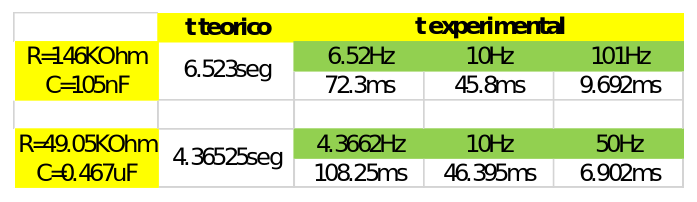
\includegraphics[scale=0.6]{ksken1.png}
\end{figure}
\item Condensador
\begin{figure}[H]
\centering
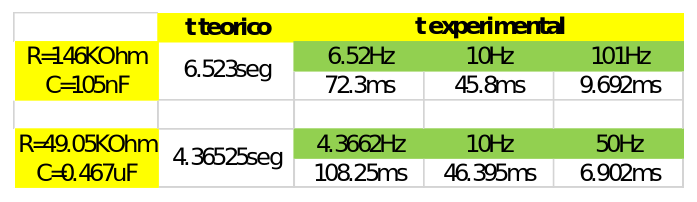
\includegraphics[scale=0.6]{ksken1.png}
\end{figure}
\end{itemize}
\begin{figure}[H]
\centering
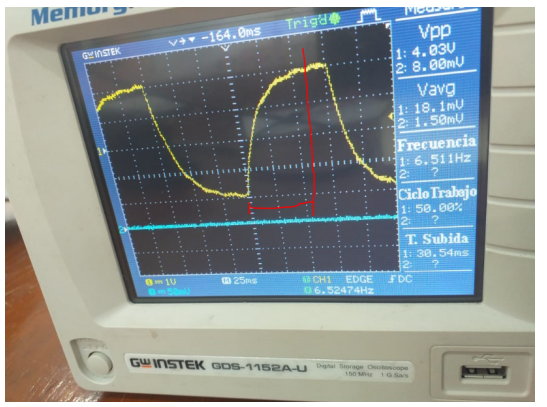
\includegraphics[scale=0.6]{ksken3.png}
\end{figure}
Para este caso las divisiones indican aproximadamente 12\,ms, que es el tau experimental
\begin{figure}[H]
\centering
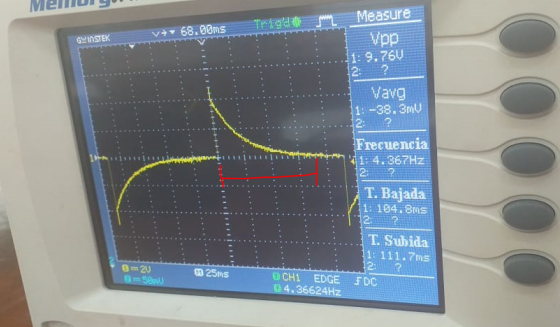
\includegraphics[scale=0.6]{ksken4.png}
\end{figure}
Para este caso las divisiones indica un tiempo de 19\,ms, que es el tau experimental.
\begin{figure}[H]
\centering
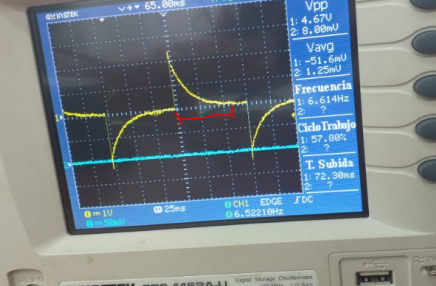
\includegraphics[scale=0.6]{ksken5.png}
\end{figure}
Para este caso el tiempo según las divisiones indica 12ms, que es el tau experimental.\\
Cuando la frecuencia aumenta el condensador tiene menos tiempo para cargarse por lo que no alcanza el valor deseado de amplitud.\\
Cálculo de error:
\begin{figure}[H]
\centering
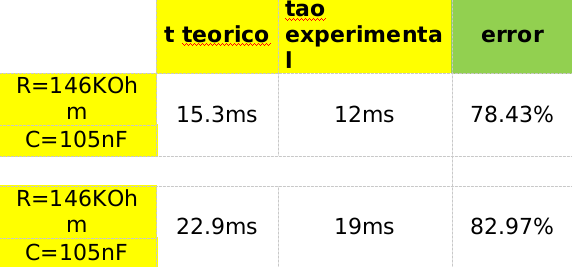
\includegraphics[scale=0.5]{ksken6.png}
\end{figure}
$$
T_{\mathrm{carga}} = \frac{1}{f}\cdot 1000 \cdot \frac{1}{2}
$$
\item Explique por qué a los circuitos utilizados se les denomina circuito derivador e integrador.
Al circuito integrador se le llama asi porque cuando llega un pulso de entrada se eleva rápidamente al máximo cargando el condensador C exponencialmente debido a la resistencia R, lo cual deforma el pulso de entrada como se muestra en la forma de onda inferior. Cuando el pulso de entrada se cae de repente acero, se descarga exponencialmente el condensador C a cero a través de la resistencia R. El proceso se repite para cada pulso de entrada que, dará la forma de onda de salida mostrada en la figura siguiente:
\begin{figure}[H]
\centering
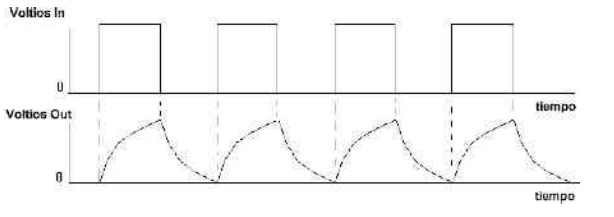
\includegraphics[scale=0.5]{ksken7.png}
\end{figure}
\begin{figure}[H]
\centering
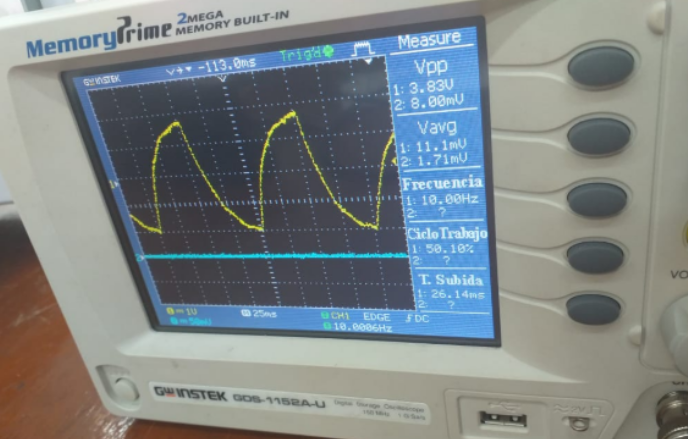
\includegraphics[scale=0.5]{ksken8.png}
\end{figure}
El circuito derivador se utiliza para detectar flancos de subida y bajada en una señal provocando una mayor diferenciación en los flancos de entrada y salida de la señal que es donde la variación con el tiempo (t) se hace más notoria.
\begin{figure}[H]
\centering
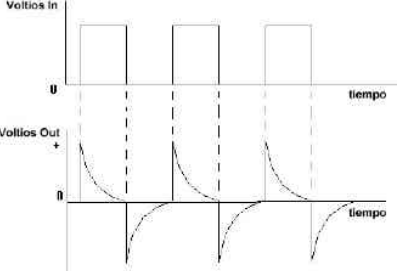
\includegraphics[scale=0.5]{ksken9.png}
\end{figure}
\begin{figure}[H]
\centering
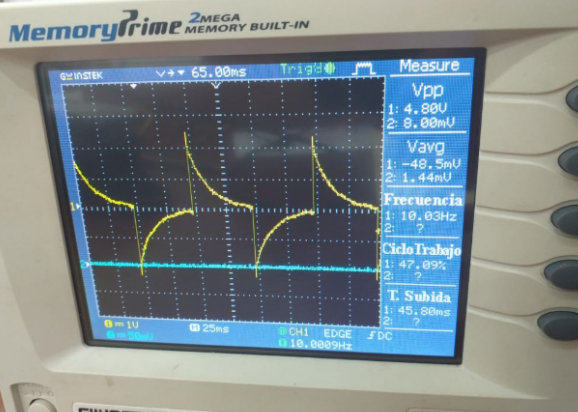
\includegraphics[scale=0.5]{ksken10.png}
\end{figure}
\item Explique la influencia que tiene la frecuencia de la señal en los circuitos integrador y derivador.\\
La influencia de la frecuencia radica básicamente en que, a alta frecuencia, es decir, cuando $\omega >> \frac{1}{RC}$ el condensador no tiene tiempo suficiente para cargarse y la tensión en los bornes permanece pequeña, el circuito es integrador.
$$
V_{R} \approx V_{in}
$$
Así:
Como,
$$
V_{c} = \frac{1}{C}\int_{0}^{t} I\,\mathrm{d}t 
$$
$$
V_{c} \approx \frac{1}{RC}\int_{0}^{t} V_{\mathrm{in}}\,\mathrm{d}t 
$$
Se obtiene.\\
La tensión en los bornes del condensador integrado se comporta como un filtro de paso-bajo.\\
Y, por otro lado, a bajas frecuencias es decir cuando $\omega < < \frac{1}{RC}$, el condensador tiene el tiempo de cargarse casi completamente, el circuito es derivador.\\
Entonces:
$$
I \approx \frac{V_{\mathrm{in}}}{1/j\omega C}
$$
$$
V_{\mathrm{in}} \approx \frac{I}{j\omega C} \approx V_{c}
$$
$$
V_{R} = IR = C\frac{\mathrm{d}\,V_{c}}{\mathrm{d}\,t}R
$$
$$
V_{R} = RC\frac{\mathrm{d}\,V_{\mathrm{in}}}{\mathrm{d}\,t}
$$
Ahora,\\
La tensión en los bornes de la resistencia derivado se comporta como un filtro de paso-alto.\\
Entonces, si la frecuencia es lo suficientemente baja, el voltaje entre las placas del capacitor (VC) aumentará y decrecerá exponencialmente, con una constante de tiempo = RC, hasta alcanzar el valor máximo de la fuente.
\begin{figure}[H]
\centering
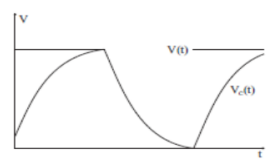
\includegraphics[scale=0.5]{land1.png}
\end{figure}
y el valor cero, respectivamente. Dicho comportamiento está esquematizado en el gráfico de la figura, donde la traza oscura representa a V (t) y la clara a VC(t).\\
Supongamos que se incrementa la frecuencia f0. El condensador en este caso podría no alcanzar el voltaje de la fuente. Como se puede ver en la figura inferior, si se continúa aumentando la frecuencia, la curva de carga y de descarga del capacitor se parecerá más A un tramo recto.
\begin{figure}[H]
\centering
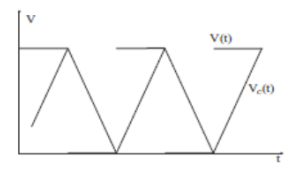
\includegraphics[scale=0.5]{land2.png}
\end{figure}
\item Explique qué sucede con la amplitud de la señal de salida cuando se varía la frecuencia de la señal de entrada.\\
En estos circuitos analizados, si la señal de entrada se aumenta, esto implica que el periodo disminuya, las amplitudes de las señales de salida, que son Vc y Vr, disminuyen. Por otro lado, si las frecuencias disminuyen, las amplitudes aumentan su valor. 
\item Encontrar analíticamente el desarrollo en serie de Fourier de la señal de entrada y las señales derivadas e integradas.\\
La serie de Fourier permite tratar cualquier función periódica como una suma finita o infinita de funciones sinusoidales relacionadas armónicamente,
\begin{figure}[H]
\centering
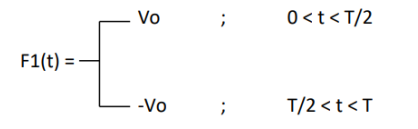
\includegraphics[scale=0.5]{land3.png}
\end{figure}
resolveré esta serie simbólicamente:\\
Para la señal de entrada se tiene una simetría de cuarto de onda impar, con lo cual el valor de la constante an=0\\
Calculamos bn con su forma trigonométrica:
$$
b_{n} = \frac{4}{T}\int V_{0}\sin \omega t \,\mathrm{d}t
$$
Si resolvemos la integral obtenemos:
$$
b_{n} = \frac{2V_{0}}{\pi} \left( \frac{1-1^{n}}{n} \right)
$$
Reemplazamos bn en la forma Fourier, reitero, an=0.
$$
F1_{t} = \sum_{n=1}^{\infty} \left[ bn \sin \omega t \right]: n = 1,3,5,7,\ldots
$$
$$
F1_{t} = \frac{2V_{0}}{\pi}\sum_{n=1}^{\infty} \left[ \left( \frac{1-1^{n}}{n} \right) \sin \omega t \right]: n = 1,3,5,7,\ldots
$$
Del mismo modo, la señal de salida es función par por lo que bn=0
$$
an = \frac{4}{T} \int \frac{V_{0}}{RC} t \cos(n\omega t)\,\mathrm{d}t
$$
Resolviendo la integral:\\
Reemplazando obtenemos:\\
Gráficamente se variará ``n''(parciales), recordemos que a mayor ``n'' hay más exactitud en las gráficas pues Fourier se ``apoya'' más a la función.
$$
F1_{t} = \frac{V_{0}t}{RC} + \frac{V_{0}T}{\pi^{2} RC} \sum_{n=1}^{\infty} \left[ \left( \frac{(-1)^{n} - 1}{n^{2}} \right) \cos (\omega t) \right]; n=0,1,2,3,\ldots
$$
\begin{figure}[H]
\centering
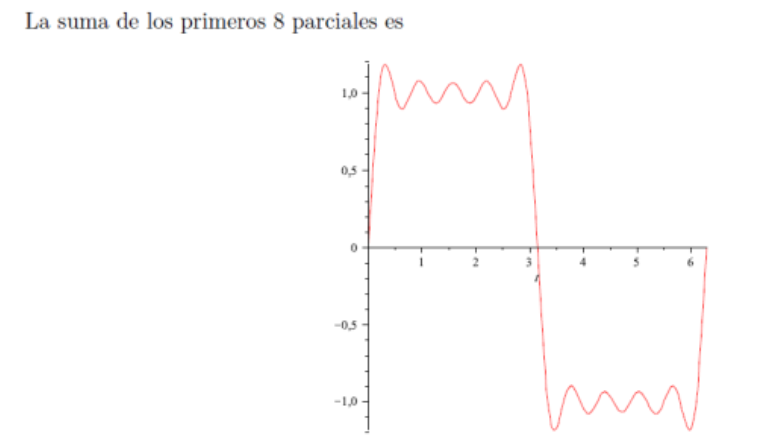
\includegraphics[scale=0.5]{land4.png}
\end{figure}
\begin{figure}[H]
\centering
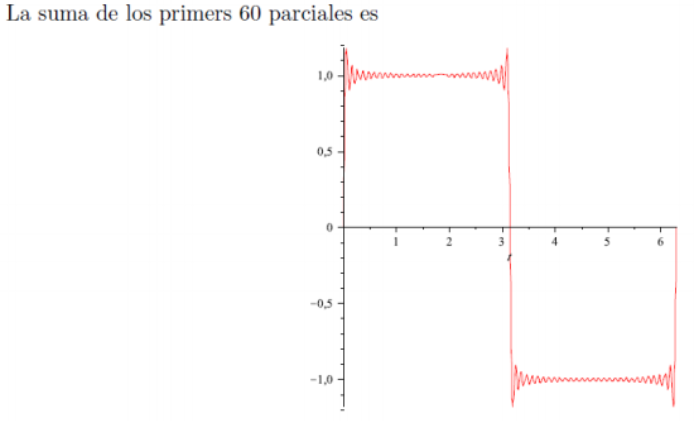
\includegraphics[scale=0.5]{land5.png}
\end{figure}
\begin{figure}[H]
\centering
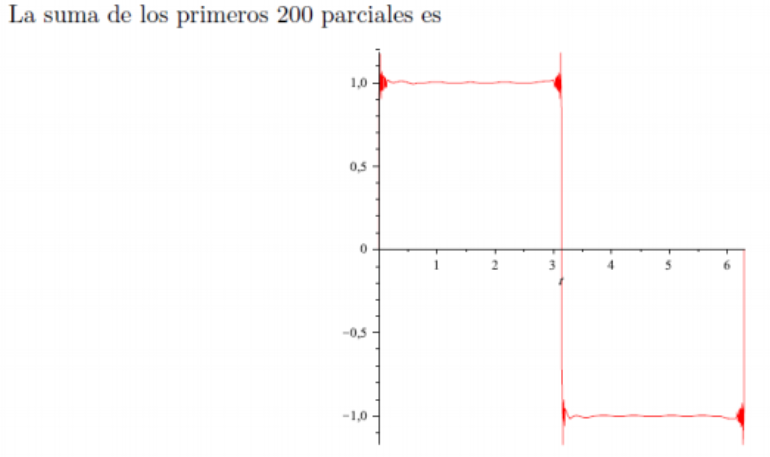
\includegraphics[scale=0.5]{land6.png}
\end{figure}
\end{enumerate}
\begin{enumerate}
\item Determine (indicando detalladamente los pasos) la ecuación diferencial del circuito mostrado.\\
De la figura, se tiene lo siguiente:
\begin{equation}
I = I_{1} + I_{2} \label{Sergod1}
\end{equation}
\begin{equation}
I_{1} = C\,V_{c}'(t) \label{Sergod2}
\end{equation}
\begin{equation}
I_{2} = \frac{V_{c}(t)}{R_{c}} \label{Sergod3}
\end{equation}
$$
V_{(t)} = R_{V}I_{(t)} + LI_{(t)}'+V_{c}(t)
$$
Acomodando:
\begin{equation}
V_{c}(t) = V_{(t)} - R_{V}I_{(t)} - LI_{(t)}' \label{Sergod4}
\end{equation}
De (\ref{Sergod2}),(\ref{Sergod3}) y (\ref{Sergod4}) en (\ref{Sergod1})
$$
I_{(t)} = CV_{c}(t)' + \frac{V_{(t)}-R_{V}I_{(t)}-LI_{(t)}'}{R_{c}}
$$
$$
I_{(t)} = CV_{c}(t)' - CR_{V}I_{(t)}' - LCI_{(t)}' + \frac{V_{(t)}-R_{V}I_{(t)}-LI_{(t)}'}{R_{c}}
$$
Agrupando los términos:
$$
I_{(t)}'+\left( \frac{1}{R_{c}C}+\frac{R_{V}}{L} \right)I_{(t)}' + \left( \frac{1}{LC} + \frac{R_{V}}{R_{C}LC} \right) I_{(t)} = \frac{V_{(t)}}{R_{c}LC} + \frac{V_{(t)}'}{L}
$$
\item Calcule analíticamente $\alpha$, $T$ y $\omega_{0}$, compare estos valores con los hallados experimentalmente, justificando las divergencias.\\
Para hallar los valores pedidos debemos tener la ecuación característica, entonces:
$$
\left[ D^{2} + \left( \frac{1}{R_{c}C} + \frac{R_{V}}{L} \right)D + \left( \frac{1}{LC} + \frac{R_{V}}{R_{c}LC} \right) \right]I_{(t)} = \frac{V_{(t)}}{R_{c}LC} + \frac{V_{(t)}'}{L}
$$
Además, sabemos que la ecuación característica debe tener la siguiente forma:
$$
\left[ D^{2} + 2\alpha D + \omega_{0}^{2} \right]X_{(t)} = f_{(t)}
$$
Por simple comparación, hallamos los valores:
$$
\alpha = \frac{1}{2} \left( \frac{1}{R_{c}C} + \frac{R_{V}}{L} \right)
$$
$$
\omega_{0} = \sqrt{\frac{1}{LC} + \frac{R_{V}}{R_{c}LC}}
$$
Además:
$$
\omega = \sqrt{\omega_{0}^{2} - \alpha^{2}}
$$
$$
\omega = \sqrt{\frac{1}{LC} - \left( \frac{R_{V}}{2L} \right)^{2} + \frac{1}{2R_{c}C}\left( \frac{R_{V}}{L} - \frac{1}{2R_{c}C} \right)} = \frac{2\pi}{T}
$$
$$
T = \frac{2\pi}{\sqrt{\frac{1}{LC} - \left( \frac{R_{V}}{2L} \right)^{2} + \frac{1}{2R_{c}C}\left( \frac{R_{V}}{L} - \frac{1}{2R_{c}C} \right)}}
$$
Para el caso 1:
$$
R_{V} = 8.57\,\mathrm{k\Omega} \hspace{20pt} L=2.5 \hspace{20pt} C = 0.0\,\mu\mathrm{F} \hspace{20pt} 26.83\,\mathrm{k\Omega}
$$
Se obtiene:
$$
\alpha = 2645.7927 \hspace{20pt} \omega_{0} = 5136.9612 \hspace{20pt} \omega = 4403.1979 \hspace{20pt} T = 1.4269\,\mathrm{ms}
$$
$$
T_{\mathrm{experimental}} = 1.6\,\mathrm{ms} \hspace*{30pt} \%\mathrm{Error} = 12.9225\%
$$
Para el caso 2:
$$
R_{V} = 8.94\,\mathrm{k\Omega} \hspace{20pt}  L =2.5 \hspace{20pt} C = 0.05\mathrm{\mu F} \hspace{20pt} R_{c} = 42.2\,\mathrm{k\Omega}
$$
Se obtiene:
$$
\alpha = 2380.417 \hspace{20pt} \omega_{0} = 4923.1054 \hspace{20pt} \omega = 4309.3597 \hspace{20pt} T = 1.458\,\mathrm{ms}
$$
$$
T_{\mathrm{experimental}} = 1.6\,\mathrm{ms} \hspace*{30pt} \%\mathrm{Error} = 9.7369\%
$$
\item ¿Qué consigue con el paso ``4''?\\
Al aumentar la resistencia del potenciómetro se disminuye las oscilaciones debido a que tanto el voltaje como la corriente a medir son más pequeñas, y por tanto las fluctuaciones menores. De esta forma se consigue una mejor visualización de la curva esperada.
\item ¿Qué función cumple $R_{c}$?\\
La corriente que pasa por la resistencia y la tensión que hay en ella están en fase debido a que la resistencia(Rc) no causa desfase. La corriente en el capacitor está adelantada con respecto a la tensión (voltaje), que es igual que decir que el voltaje está retrasado con respecto a la corriente.
\item ¿Qué diferencias observa en los pasos 3,4 y 5 y a qué se deben estas diferencias?\\
Los cambios se deben a que la magnitud de la corriente alterna total es igual a la suma de las corrientes que pasan por la corriente y el condensador y se obtiene con ayuda de las siguientes fórmulas:
\begin{itemize}
\item Magnitud de la corriente (AC) total:
$$
I_{t} =  \sqrt{I_{r}^{2} + I_{c}^{2}}
$$
\item Ángulo de desfase $\theta$:
$$
\theta = \arctan \frac{-I_{c}}{I_{r}}
$$
Al ir quitando la resistencia $R_{c}$ y $R$ el sistema varia porque sus intensidades cambian y la diferencia de voltaje también en los 3 circuitos del paso 3, 4 y 5.
\end{itemize}
\end{enumerate}
\chapter{Conclusiones y recomendaciones}
\begin{enumerate}
\item Se observó que la frecuencia efectiva para que las gráficas deseadas salgan en el osciloscopio se calculan previamente con la fórmula 
\item Se tuvo que medir todas las resistencias previamente y afortunadamente en nuestro circuito estaba midiendo exactamente lo indicado.
\end{enumerate}
\begin{thebibliography}{99}  %%%este es un contador para el número de bibliografías utilizados.
\addcontentsline{toc}{chapter}{Bibliograf\'{\i}a} %%% Para introducir la bibliografía en el índice.
%\bibitem{Rahman}{Rahman,Aminur y Doe, Hidekazu; ``Ion transfer of tetraalkylammonium cations at an interface between 
%frozen aqueous solution and 1,2-dichloroethane".{\em{Journal of Electroanalytical Chemistry}} {\bfseries 424},159,(1997).}
\bibitem{Gro}{Boylestad, Robert M. ``Introducción al análisis de circuitos''. {\em{Pearson}}}
\bibitem{Gro}{Sadiku, Matthew N. ``Fundamemtos de circuitos eléctricos''. {\em{Mc Graw Hill}}}
%\bibitem{Ding}{Ding, Zhifeng. ``Spectroelectrochemistry and photoelectrochemistry of charge transfer at liquid/liquid
%interfaces". {\em {Tesis, EPFL,}}(1999).}
%\bibitem{AL}{Alonso, Jose M. \em{Técnicas de mecanizado 1}}
%\bibitem{AL}{Alonso, Jose M. ``Técnicas de mecanizado 1". {\em{Paraninfo}} {\bfseries España-Madrid}, 6-20, (2001).}
%\bibitem{Samec2}{Samec Z., Lhotsky A., Jänchenová H., y Marecek, V. ``Interfacial tension and impedance measurements
%of interfaces between two inmiscible electrolyte solutions". {\em{Journal of Electroanalytical Chemistry}} {\bfseries
%43}, 47, (2000).}
%\bibitem{Day}{Day R.A. y Underwood A.L. {\textit{Química Analítica Cuantitativa}},5ºed. Prentice-Hall, México, 1998. 45-48.}
%\bibitem{Keyser}{Farah Abud, Michel. ``Determinación de la vida útil en herramientales de corte endurecido por el proceso de borurización en pasta''. {\em{Instituto tecnológico y de estudios superiores de Monterrey}}}
%\bibitem{Zolotorevski}{Escalona, I. ``Máquinas: herramientas por arranque de viruta.''.{\em{El Cid Editor.}}}
%\bibitem{Lasheras}{Lasheras. ``Tecnología de los Materiales Industriales''.} 
%\bibitem{Dieter}{Dieter. ``Metalurgia mecánica''.}
%\bibitem{Apraiz}{Apraiz, J. ``Tratamiento Térmico de los Aceros''.}
%\bibitem{Smith}{Smith, William F. y Ph.D. Hashemi, Javad ``Ciencia e ingeniería de materiales". {\em{
%Madrid: McGraw-Hill, Interamericana de España.}} 570, (2004).} 
%\bibitem{Callister}{Callister, William D. y Rethwisch, David G. ``Introducción a la ingeniería de los materiales''. %{\em{Barcelona Reverté.}}, 960, (2007).} 
%\bibitem{Askeland}{Askeland, Donald R., Pradeep P. Phulé y Wright, Wendelin J. ``Ciencia e ingeniería de los materiales''.{\em{México, D.F. Internacional Thomson Editores.}} {\textit{$6^{ta}$ edición}}, 1004, (2012).}
%\bibitem{HARDBANDING}{Tabla de conversión de escala de durezas. \begin{verbatim}http://%hardbandingsolutions.com/postle_sp/hardness.php
%\end{verbatim}}
%\bibitem{HE}{Fresadora. \begin{verbatim} http://lizdenbow.blogspot.com/
%\end{verbatim}}
%\bibitem{ASTM}{Normas ASTM.}
%\bibitem{NTP}{Normas NTP.}
\end{thebibliography}
\end{document}